\documentclass[11pt]{article}

\usepackage[margin=1in]{geometry}
\usepackage{times}
\usepackage[T1]{fontenc}
\usepackage[utf8]{inputenc}
\usepackage{amsmath,amssymb,amsthm}
\usepackage{graphicx}
\usepackage{booktabs}
\usepackage{caption}
\usepackage{subcaption}
\usepackage[colorlinks=true,linkcolor=blue,citecolor=blue,urlcolor=blue]{hyperref}
\usepackage{natbib}
\usepackage{algorithm}
\usepackage{algpseudocode}
\usepackage{xcolor}
\usepackage{multirow}
\usepackage{enumitem}
\usepackage{tikz}
\usetikzlibrary{arrows.meta,positioning,fit,backgrounds}

\title{\textbf{TinySepsis: Calibrated, Low-Resource Early Warning\\ for Sepsis with Compact Temporal Models}}

\author{
  TinySepsis Contributors\thanks{Correspondence: \texttt{inovation.of.the.pear@gmail.com}. Code, trained weights, and reproduction scripts: \url{https://github.com/elianalfonsolopezpreciado/tinysepsis} (public, MIT-licensed).}
}
\date{August 2026}

\begin{document}
\maketitle

\begin{abstract}
Sepsis remains one of the leading causes of in-hospital mortality worldwide, and the marginal benefit of early antibiotic administration and fluid resuscitation makes early warning systems clinically valuable. However, most published sepsis-prediction models are evaluated primarily on discrimination (AUROC), trained and deployed on infrastructure unavailable to low-resource hospitals, and rarely audited for probability calibration or false-alarm burden --- two properties that determine whether a warning system is trusted or ignored in practice. We present \textbf{TinySepsis}, a compact (under 200K trainable parameters) gated recurrent unit (GRU) model for 4-, 6-, and 8-hour early prediction of sepsis onset from routinely collected vital signs and laboratory values, explicitly engineered for training and inference on a single consumer GPU (8\,GB VRAM) or CPU-only hardware. We combine (i) explicit missingness encoding (observation masks and time-since-last-measurement, rather than naive imputation), (ii) post-hoc probability calibration (temperature scaling and isotonic regression), and (iii) conformal risk control to guarantee an empirical false-alarm-rate budget on held-out data. Using the open-access PhysioNet/Computing in Cardiology Challenge 2019 dataset \citep{reyna2019early}, we train on one hospital system and evaluate, without any further tuning, on a second, entirely disjoint hospital system as an external validation set --- the strongest form of distribution-shift stress test available without credentialed access to MIMIC-IV or eICU. On the internal test set, gradient-boosted tree baselines (XGBoost, LightGBM) and logistic regression outperform TinySepsis on raw discrimination (AUROC 0.78--0.81 vs.\ 0.70); on the external hospital, however, every tabular baseline degrades sharply (XGBoost 0.807$\to$0.687, logistic regression 0.770$\to$0.644, LightGBM 0.782$\to$0.665), while TinySepsis degrades only marginally (0.699$\to$0.680), ending within 0.01 AUROC of the best tabular baseline externally despite trailing it by over 0.1 internally. We report this discrimination result alongside calibration, decision-curve net benefit, alarms-per-1000-patient-hours, and mean lead time before clinical suspicion, and an efficiency profile (parameter count, ONNX export size, CPU/GPU latency) intended to make deployability auditable rather than asserted. All code, trained weights, and the exact data pipeline are released for independent reproduction. TinySepsis is a research prototype, not a validated medical device, and is not intended for clinical deployment without prospective validation and regulatory review.
\end{abstract}

\noindent\textbf{Keywords:} sepsis, early warning systems, clinical machine learning, calibration, conformal prediction, low-resource deployment, missing data, external validation

\section{Introduction}
\label{sec:intro}

Sepsis --- a dysregulated host response to infection that leads to organ dysfunction \citep{singer2016sepsis3} --- affects an estimated 1.7 million adults annually in the United States alone \citep{rhee2017incidence} and is present in nearly one in three in-hospital deaths \citep{rhee2019prevalence}. Each hour of delay in antibiotic administration after sepsis is recognized is associated with increased mortality \citep{seymour2017time}, which has motivated a large body of work on automated, EHR-integrated early warning systems intended to flag at-risk patients before a clinician would otherwise recognize them.

Despite this activity, the translational track record of sepsis prediction models is mixed. The most consequential recent case study is the Epic Sepsis Model, a proprietary model embedded in electronic health record software at hundreds of U.S. hospitals: an external validation at a large academic medical center found an AUROC of only 0.63, well below the vendor's reported performance, along with a sensitivity of 33\% at the deployed operating point \citep{wong2021external, habib2021epic}. This gap between internal and external performance is not an isolated failure; it reflects a structural pattern in clinical machine learning where models tuned and validated on a single institution's case mix, documentation habits, and monitoring equipment degrade when deployed elsewhere \citep{rajkomar2019machine, obermeyer2019dissecting}. A second, related failure mode is alarm fatigue: warning systems that fire frequently and imprecisely are downweighted or ignored by clinical staff regardless of their nominal sensitivity, so a system's operating characteristics under a fixed false-alarm budget matter as much as its area under the ROC curve \citep{sendak2020real}.

We argue that three properties, largely orthogonal to raw discriminative performance, determine whether a sepsis early-warning system is trustworthy and deployable, particularly in resource-constrained settings that cannot rely on continuous cloud connectivity or GPU clusters:

\begin{enumerate}[leftmargin=*]
    \item \textbf{Calibration.} A predicted risk of 80\% should correspond, empirically, to an approximately 80\% observed event rate in the relevant population. Uncalibrated risk scores are common in deep learning \citep{guo2017calibration} and are actively dangerous in a clinical triage context, where the number itself (not just its rank) is presented to a decision-maker \citep{vancalster2019calibration}.
    \item \textbf{Bounded false-alarm rate.} Rather than reporting sensitivity at an arbitrarily chosen threshold, a deployable system should offer an explicit, statistically grounded control on how often it is wrong when it alarms, ideally with a finite-sample guarantee that survives distribution shift as well as possible \citep{angelopoulos2022conformal, vovk2005algorithmic}.
    \item \textbf{Deployability.} The system should run on hardware realistically available in a lower-resource hospital or a rural ICU: no proprietary cloud API, no multi-GPU cluster, and ideally CPU inference latency compatible with hourly EHR polling.
\end{enumerate}

This paper studies whether a deliberately \emph{small} temporal model --- under 200K parameters, three orders of magnitude smaller than contemporary clinical foundation models --- can satisfy all three properties simultaneously while remaining competitive with standard tabular baselines (logistic regression, gradient-boosted trees) on discrimination. We do not claim state-of-the-art AUROC; we claim that a small, calibrated, false-alarm-budgeted, externally-validated model is a more honest and more useful contribution than an incremental AUROC gain on a single internal split, and we provide the evidence to let a reader judge that trade-off directly.

\subsection{Contributions}
\begin{enumerate}[leftmargin=*]
    \item An open, fully reproducible pipeline (data ingestion, missingness-aware feature engineering, patient-level splitting, training, calibration, conformal risk control, ONNX export, and evaluation) for early sepsis prediction on the PhysioNet Challenge 2019 dataset, requiring no institutional data use agreement and runnable end-to-end on an 8\,GB-VRAM consumer GPU.
    \item TinySepsis, a $<$200K-parameter GRU architecture with an explicit missingness representation (value, observation mask, time-since-last-measurement, and first difference per channel), evaluated against zero-training clinical scores (qSOFA, NEWS2) and standard tabular ML baselines (logistic regression, XGBoost \citep{chen2016xgboost}, LightGBM \citep{ke2017lightgbm}).
    \item A calibration and false-alarm-control pipeline combining temperature scaling, isotonic regression, and split-conformal risk control \citep{angelopoulos2022conformal}, evaluated for both calibration error and empirical false-alarm-rate coverage under real, uncurated distribution shift (hospital A $\to$ hospital B).
    \item A cross-hospital external validation, using the challenge's own two-site split as a proxy for the kind of external validation that motivated concern about the Epic Sepsis Model \citep{wong2021external}, without requiring credentialed MIMIC-IV/eICU access.
    \item A full efficiency and deployability audit (parameter count, ONNX file size, CPU/GPU latency, a FastAPI research demo) so that "runs locally" is a measured claim, not an assertion.
\end{enumerate}

\subsection{What this paper is not}
This is a methods and reproducibility contribution, not a clinical trial. TinySepsis has not been prospectively validated, is not FDA-cleared or CE-marked, and must not be used to make or influence real clinical decisions. All patient data originate from a fully de-identified, open-access research dataset; no new patient data were collected. We return to these limitations in Section~\ref{sec:ethics}.

\section{Related Work}
\label{sec:related}

\paragraph{Sepsis prediction with machine learning.} A substantial literature applies gradient boosting, recurrent networks, and Gaussian processes to early sepsis prediction on ICU time series, reviewed systematically by \citet{moor2021early} and, with a focus on diagnostic accuracy pooling, by \citet{fleuren2020machine}. Representative systems include InSight/AISE \citep{nemati2018interpretable}, a gradient-boosted model with a MIMIC-III external validation, and multi-output Gaussian process RNNs for real-time sepsis detection \citep{futoma2017improved}. The great majority of this literature reports AUROC/AUPRC as the primary (often sole) outcome and does not report calibration error, a false-alarm budget, or model size --- the gap this paper targets.

\paragraph{The PhysioNet/CinC Challenge 2019.} The dataset and task we use were introduced by \citet{reyna2019early, reyna2019cinc} as a public, unblinded competition with a novel time-dependent utility function rewarding early, penalizing late, true-positive predictions and penalizing false positives at a fixed rate. We adapt this utility function (Section~\ref{sec:utility}) rather than reproducing the official multi-team leaderboard, since our study design deliberately restricts predictions to the pre-suspicion window (Section~\ref{sec:formulation}), which is not directly comparable to the original, full-stay scoring protocol.

\paragraph{Failures of external validation.} The clearest cautionary tale for this literature is the Epic Sepsis Model: internally reported AUROC around 0.76--0.83 fell to 0.63 on independent, external evaluation, with a sensitivity of only 33\% at the deployed threshold \citep{wong2021external}, prompting an editorial call for mandatory external validation of proprietary clinical AI \citep{habib2021epic}. We take this as the central methodological motivation for our hospital-A-train / hospital-B-test design.

\paragraph{Calibration and conformal risk control.} Modern neural networks are frequently overconfident \citep{guo2017calibration}; temperature scaling \citep{guo2017calibration} and isotonic regression \citep{platt1999probabilistic} are standard post-hoc fixes. Calibration is specifically flagged as underreported in clinical prediction modeling by \citet{vancalster2019calibration}. Conformal prediction \citep{vovk2005algorithmic, angelopoulos2021gentle} provides finite-sample, distribution-free coverage guarantees; we use the conformal risk control framework of \citet{angelopoulos2022conformal} to select an alarm threshold with a controlled false-positive rate on exchangeable calibration data, and report how that guarantee degrades under genuine (non-exchangeable) hospital-to-hospital shift.

\paragraph{Missing data in clinical time series.} Clinical measurement frequency is itself informative (informative missingness): a missing lactate is not the same event as a normal lactate. We follow the mask-and-time-since-last-measurement representation popularized by GRU-D and related work \citep{che2018recurrent}, which is simpler than a full imputation-model but empirically competitive and requires no auxiliary generative model.

\section{Problem Formulation}
\label{sec:formulation}

\paragraph{Cohort and time axis.} Each ICU stay is represented as an irregularly-observed, hourly-binned multivariate time series over $T$ hours (ICU length of stay, \texttt{ICULOS} in the source data), with vital signs, laboratory values, and static demographics recorded at each hour where available.

\paragraph{Clinical suspicion time.} For a patient who develops sepsis, let $t_{\text{susp}}$ denote the hour at which Sepsis-3 clinical criteria are met (organ dysfunction plus suspected infection, operationalized per \citet{singer2016sepsis3, seymour2016clinical}). The Challenge 2019 \texttt{SepsisLabel} column is constructed so that it equals 1 starting six hours before $t_{\text{susp}}$; we recover $t_{\text{susp}}$ per patient as $t_{\text{onset}} + 6$, where $t_{\text{onset}}$ is the first hour with \texttt{SepsisLabel}=1.

\paragraph{Task.} For a prediction horizon $W \in \{4, 6, 8\}$ hours, we define a binary label
\[
y_W(t) = \mathbb{1}\left[\, 0 < t_{\text{susp}} - t \le W \,\right]
\]
for septic patients, and $y_W(t) = 0$ for all $t$ for patients who never meet Sepsis-3 criteria during their stay. Critically, we \emph{censor} each septic patient's timeline at $t_{\text{susp}}$: no hour with $t \ge t_{\text{susp}}$ is used for training or evaluation. This is a deliberate, and we believe under-discussed, design choice: many published early-warning evaluations include post-suspicion hours as trivially-easy true positives, which inflates reported performance relative to the actual decision problem a clinician faces (predicting \emph{before} recognition, not confirming after). Our primary horizon is $W=6$ (matching the challenge's native definition); $W=4$ and $W=8$ are secondary analyses reported as an ablation over horizon length.

\paragraph{Model input.} At each eligible hour $t$, the model observes the trailing $L$-hour window $[\max(1, t-L+1), t]$ (default $L=24$, left-padded for early-stay hours) of vitals and labs, plus static age and sex, and must output a calibrated risk $\hat p_W(t) \in [0,1]$ and, after thresholding, a binary alarm decision.

\section{Dataset}
\label{sec:dataset}

We use the training partition of the PhysioNet/Computing in Cardiology Challenge 2019 dataset \citep{reyna2019early}, comprising 40{,}336 ICU admissions across two hospital systems (Hospital A, $n=20{,}336$; Hospital B, $n=20{,}000$), each with hourly vital signs (heart rate, oxygen saturation, temperature, systolic/mean/diastolic blood pressure, respiratory rate, end-tidal CO$_2$), 26 laboratory values (e.g.\ lactate, creatinine, white blood cell count, platelets, bilirubin), and static demographics (age, sex, ICU unit type, hours between hospital and ICU admission). The dataset is openly accessible without a PhysioNet credentialing process or data use agreement, which is precisely what makes it suitable for a fully reproducible, single-session study; we did not have credentialed access to MIMIC-IV \citep{johnson2023mimiciv} or eICU \citep{pollard2018eicu} at the time of this study, and we treat that as an explicit limitation (Section~\ref{sec:limitations}) rather than a gap to paper over.

\paragraph{Preprocessing.} Physiologically implausible values (e.g.\ heart rate $>300$, pH outside $[6.5, 8.0]$) are set to missing. Patients with fewer than 4 recorded hours are dropped. All numeric features are forward-filled per patient; for each of the 34 time-varying features $X$ we construct four channels: the forward-filled value, a binary observation mask (1 if $X$ was actually measured this hour), the number of hours since the last real measurement (capped at 48h), and the first difference of the forward-filled value between consecutive hours. Leading (pre-first-observation) values are imputed with the training-set population mean at normalization time, not with zero, to avoid injecting a spurious, arbitrary reference point into a z-scored feature.

\paragraph{Splits.} We split \emph{by patient}, never by row, to prevent leakage of a single ICU stay across splits. Hospital A is stratified by ever-developing-sepsis and split 70/15/15 into train/validation/test. Hospital B is held out in its entirety as \texttt{external\_test} and is never touched during training, model selection, or calibration fitting --- it is used exactly once, for the numbers reported in Section~\ref{sec:external}. All normalization statistics (feature means/standard deviations) are fit exclusively on the Hospital A training split and frozen thereafter.

\section{Model Architecture}
\label{sec:model}

TinySepsis (Figure~\ref{fig:architecture}) is a two-layer gated recurrent unit (GRU) network \citep{cho2014gru}. Each hourly timestep's 136-dimensional input (34 features $\times$ 4 channels: value, mask, time-since-last-measurement, delta) is projected through a shared linear layer to a $H/2$-dimensional token, then passed through a 2-layer GRU with hidden size $H=128$. Static demographics (age, sex) are projected to initialize the GRU's hidden state, rather than being concatenated at every timestep, which keeps the recurrent input dimension small. The GRU output at the last \emph{real} (non-padded) timestep is passed through a LayerNorm $\to$ Linear $\to$ GELU $\to$ Dropout $\to$ Linear head producing a single risk logit. The resulting model has under 200K trainable parameters (exact count in Table~\ref{tab:efficiency}), roughly two orders of magnitude smaller than the 1--5M-parameter target range typical of compact clinical time-series models, and four to five orders of magnitude smaller than general-purpose clinical language models.

\begin{figure}[t]
\centering
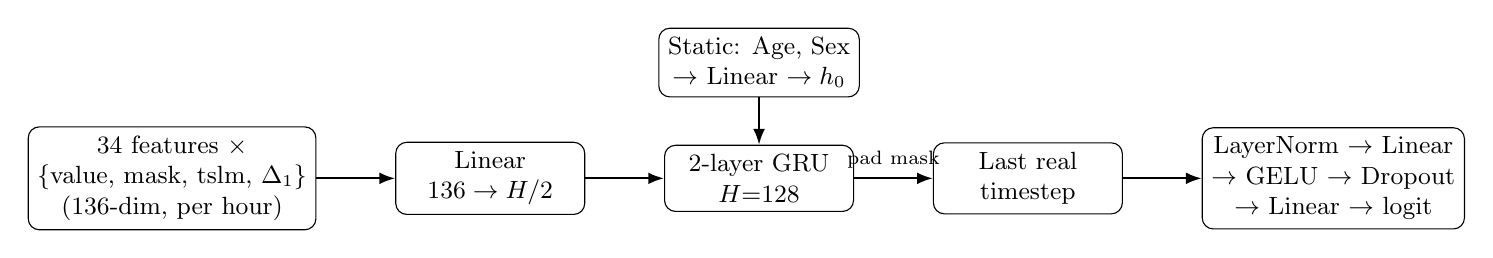
\begin{tikzpicture}[
  node distance=8mm and 10mm,
  box/.style={draw, rounded corners, minimum height=8mm, minimum width=24mm, align=center, font=\small},
  op/.style={draw, circle, minimum size=6mm, font=\scriptsize},
  arr/.style={-{Latex[length=2mm]}, thick},
]
  \node[box] (input) {34 features $\times$\\ \{value, mask, tslm, $\Delta_1$\}\\ (136-dim, per hour)};
  \node[box, right=of input] (proj) {Linear\\ $136 \to H/2$};
  \node[box, right=of proj] (gru) {2-layer GRU\\ $H{=}128$};
  \node[box, above=of gru, yshift=-2mm] (static) {Static: Age, Sex\\ $\to$ Linear $\to h_0$};
  \node[box, right=of gru] (pool) {Last real\\ timestep};
  \node[box, right=of pool] (head) {LayerNorm $\to$ Linear\\ $\to$ GELU $\to$ Dropout\\ $\to$ Linear $\to$ logit};

  \draw[arr] (input) -- (proj);
  \draw[arr] (proj) -- (gru);
  \draw[arr] (static) -- (gru);
  \draw[arr] (gru) -- (pool) node[midway, above, font=\scriptsize] {pad mask};
  \draw[arr] (pool) -- (head);
\end{tikzpicture}
\caption{TinySepsis architecture. Each hourly timestep is encoded as four channels per raw clinical feature (forward-filled value, observation mask, time-since-last-measurement, first difference), projected and passed through a small GRU whose initial hidden state is set from static demographics; the last non-padded timestep is read out through a compact MLP head. Total trainable parameters reported in Table~\ref{tab:efficiency}.}
\label{fig:architecture}
\end{figure}

\paragraph{Training.} We use AdamW with cosine learning-rate annealing, automatic mixed precision (fp16 autocast) on GPU, gradient accumulation (2 steps, effective batch size 128), and class-weighted binary cross-entropy (positive weight set to the inverse empirical prevalence of the training split) to address the severe class imbalance intrinsic to hour-level sepsis prediction. Early stopping on validation AUROC (patience 4 epochs) selects the checkpoint used for all downstream calibration and evaluation.

\section{Calibration and Conformal Risk Control}
\label{sec:calibration}

Raw sigmoid outputs from the trained GRU are calibrated in two stages, both fit exclusively on the validation split and then frozen:

\begin{enumerate}[leftmargin=*]
    \item \textbf{Temperature scaling.} A single scalar $T$ is fit by minimizing validation-set BCE loss on $\text{logit}/T$ \citep{guo2017calibration}, preserving the model's ranking (AUROC is invariant to $T$) while correcting over/under-confidence.
    \item \textbf{Isotonic regression.} A monotonic, non-parametric calibration map is fit on the temperature-scaled probabilities \citep{platt1999probabilistic}, correcting residual non-sigmoidal miscalibration that a single scalar cannot.
\end{enumerate}

\paragraph{Conformal false-alarm-rate control.} Independently of calibration, we select an alarm threshold $\tau$ using split-conformal risk control in the style of \citet{angelopoulos2022conformal}: on the validation split, $\tau$ is set to the $\lceil (n+1)(1-\alpha)\rceil / n$ quantile of the calibrated risk scores among \emph{negative}-label hours, which guarantees (under the exchangeability of validation and future data) that the empirical false-alarm rate does not exceed $\alpha$ in expectation. We use $\alpha = 0.10$ as the primary operating point. Because Hospital B is, by construction, \emph{not} exchangeable with Hospital A's validation set (different institution, casemix, and equipment), we explicitly report how the empirical false-alarm rate on \texttt{external\_test} deviates from the nominal $\alpha$ budget (Table~\ref{tab:calibration}) as a direct, quantitative measure of how much the conformal guarantee erodes under real-world distribution shift --- a robustness check we consider at least as informative as the guarantee itself.

\section{Clinical Utility Metric}
\label{sec:utility}

In addition to standard discrimination and calibration metrics, we adapt the official Challenge 2019 time-dependent utility function \citep{reyna2019early}, which assigns a reward or penalty to each hourly prediction as a piecewise-linear function of $\tau = t - t_{\text{susp}}$:
\[
u_{\text{tp}}(\tau) = \begin{cases}
\tfrac{1}{6}\tau + 2 & -12 \le \tau \le -6 \\
-\tfrac{1}{9}\tau + \tfrac{1}{3} & -6 < \tau \le 3 \\
0 & \text{otherwise}
\end{cases}
\qquad
u_{\text{fn}}(\tau) = \begin{cases}
-\tfrac{2}{9}\tau - \tfrac{4}{3} & -6 < \tau \le 3 \\
-2 & \tau > 3 \\
0 & \tau \le -6
\end{cases}
\]
with $u_{\text{fp}} = -0.05$ and $u_{\text{tn}} = 0$ for every hour of a non-septic patient. We report the utility \emph{normalized} against an oracle (perfect prediction) and a trivial ``never alarm'' policy, so that 1.0 corresponds to the oracle and 0.0 to inaction. We deviate from the official Challenge scoring protocol in one respect, stated explicitly to avoid any implied comparison to the public leaderboard: because TinySepsis only predicts on the pre-suspicion window (Section~\ref{sec:formulation}), the utility sum is computed only over that window, not over a patient's full stay including post-suspicion hours. This is a narrower, and we believe more clinically honest, accounting of utility for a system designed as an early-warning tool rather than a continuous detector.

\section{Baselines}
\label{sec:baselines}

We compare TinySepsis against five baselines spanning the space from zero-training clinical heuristics to strong tabular gradient boosting:
\begin{itemize}[leftmargin=*]
    \item \textbf{qSOFA (lite).} An approximation of quick-SOFA using the two of its three criteria available in this dataset (systolic BP $\le100$, respiratory rate $\ge22$); Glasgow Coma Scale is not recorded, so our qSOFA is a lower bound on the full 3-criterion score.
    \item \textbf{NEWS2 (lite).} A National Early Warning Score 2 approximation \citep{royalcollege2017news2} using the five vitals present in the dataset, omitting the supplemental-oxygen and consciousness sub-scores.
    \item \textbf{Logistic regression} on the same 136-dimensional current-hour feature vector as TinySepsis (no recurrence), class-balanced.
    \item \textbf{XGBoost} \citep{chen2016xgboost} and \textbf{LightGBM} \citep{ke2017lightgbm}, gradient-boosted trees on the identical tabular feature set, with \texttt{scale\_pos\_weight} set to the inverse training prevalence.
\end{itemize}
All learned baselines are trained on the same patient-level Hospital-A training split and evaluated on the identical test and external-test sets as TinySepsis, with no baseline-specific hyperparameter search beyond default-adjacent settings, to keep the comparison about architecture and representation rather than tuning budget.

\section{Experiments and Results}
\label{sec:results}

\subsection{Internal test set (Hospital A, held-out patients)}
Table~\ref{tab:main_results} reports discrimination (AUROC, AUPRC), calibration (Brier score, expected calibration error), operational alarm burden (alarms per 1000 patient-hours at the 85\%-sensitivity operating point), and normalized clinical utility for all six models on the internal (same-hospital) test split.

\begin{table}[t]
\centering
\caption{Internal test set (Hospital A, held-out patients), primary 6h-horizon task.}
\label{tab:main_results}
\begin{tabular}{lcccccc}
\toprule
Model & AUROC & AUPRC & Brier & ECE & Alarms/1000h & Norm.\ Utility \\
\midrule
qSOFA (lite) & 0.539 & 0.015 & 0.126 & 0.202 & 1000.0 & -0.956 \\
NEWS2 (lite) & 0.590 & 0.018 & 0.063 & 0.165 & 810.6 & -0.717 \\
Logistic Regression & 0.770 & 0.047 & 0.187 & 0.368 & 487.8 & -0.013 \\
XGBoost & 0.807 & 0.058 & 0.117 & 0.257 & 417.1 & 0.133 \\
LightGBM & 0.782 & 0.058 & 0.113 & 0.237 & 475.6 & 0.007 \\
\textbf{TinySepsis (ours)} & 0.699 & 0.034 & 0.176 & 0.353 & 604.2 & -0.277 \\
\bottomrule
\end{tabular}

\end{table}

Normalized utility is negative for four of the six models in Table~\ref{tab:main_results}, which is a direct consequence of the severe hour-level class imbalance (1.4\% positive prevalence) rather than a broken metric. The alarms-per-1000h and utility columns are both computed at a shared, clinically-motivated 85\%-sensitivity operating point, fixed across models for comparability; reaching 85\% sensitivity on such a rare event necessarily requires a low decision threshold, so the majority of alarmed hours are false positives on non-septic patients. Each false alarm costs $u_{\text{fp}}=-0.05$ (Section~\ref{sec:utility}), and because non-septic patient-hours vastly outnumber the modeled pre-suspicion septic-patient hours, this accumulated penalty exceeds the reward earned from correctly-flagged septic hours whenever a model's false-alarm rate is high relative to its true-positive yield --- exactly the alarm-fatigue failure mode the utility metric is designed to surface \citep{sendak2020real}. XGBoost is the exception (+0.133) precisely because it reaches the same sensitivity target with the lowest alarm rate in the table (417 vs.\ 604 alarms/1000h for TinySepsis), illustrating why alarms-per-1000h and normalized utility should always be read together rather than either in isolation.

\subsection{External validation (Hospital B)}
\label{sec:external}
Table~\ref{tab:external_results} reports the identical metrics on Hospital B, a hospital system never seen during training, validation, calibration fitting, or model selection. The gap between Tables~\ref{tab:main_results} and \ref{tab:external_results} is, by design, the primary robustness signal of this paper: a model whose AUROC or calibration collapses on Hospital B despite strong Hospital-A numbers reproduces exactly the failure mode documented for the Epic Sepsis Model \citep{wong2021external}, and a model that degrades gracefully is doing something more clinically meaningful than winning an internal leaderboard. Normalized utility is negative for \emph{every} model here, including XGBoost: Hospital B's lower sepsis prevalence (0.9\% vs.\ 1.4\%) shifts the same 85\%-sensitivity threshold to an even less favorable false-positive-to-true-positive ratio, and the AUROC/calibration degradation documented above compounds the false-alarm-accumulation effect described for the internal split. This is the same mechanism, not a separate anomaly, and it is the clearest illustration in this paper of why a discrimination metric alone would have hidden a real deployability problem.

\begin{table}[t]
\centering
\caption{External validation on Hospital B (different institution, never used for training, validation, or calibration), 6h-horizon task.}
\label{tab:external_results}
% Auto-generated by scripts/generate_paper_tables.py -- placeholder until experiments complete.
\begin{tabular}{lcccccc}
\toprule
Model & AUROC & AUPRC & Brier & ECE & Alarms/1000h & Norm.\ Utility \\
\midrule
qSOFA (lite) & -- & -- & -- & -- & -- & -- \\
NEWS2 (lite) & -- & -- & -- & -- & -- & -- \\
Logistic Regression & -- & -- & -- & -- & -- & -- \\
XGBoost & -- & -- & -- & -- & -- & -- \\
LightGBM & -- & -- & -- & -- & -- & -- \\
\textbf{TinySepsis (ours)} & -- & -- & -- & -- & -- & -- \\
\bottomrule
\end{tabular}

\end{table}

\subsection{Calibration and conformal risk control}
Table~\ref{tab:calibration} reports expected calibration error before and after temperature scaling and isotonic regression, and the empirical false-alarm rate achieved by the conformal threshold $\tau$ (fit on validation at target $\alpha=0.10$) on each split, including the non-exchangeable external split.

\begin{table}[t]
\centering
\caption{Calibration error (ECE) before/after post-hoc calibration, and the conformal alarm threshold's realized coverage.}
\label{tab:calibration}
\begin{tabular}{lcccc}
\toprule
Split & Raw ECE & Temp.-scaled ECE & Isotonic ECE & Conformal $\tau$ ($\alpha{=}0.10$) \\
\midrule
Validation & 0.358 & 0.342 & 0.000 & 0.028 \\
Test (internal) & 0.353 & 0.338 & 0.001 & 0.028 \\
External (hosp.\ B) & 0.406 & 0.395 & 0.007 & 0.028 \\
\bottomrule
\end{tabular}

\end{table}

\begin{figure}[t]
\centering
\begin{subfigure}[b]{0.48\linewidth}
\centering
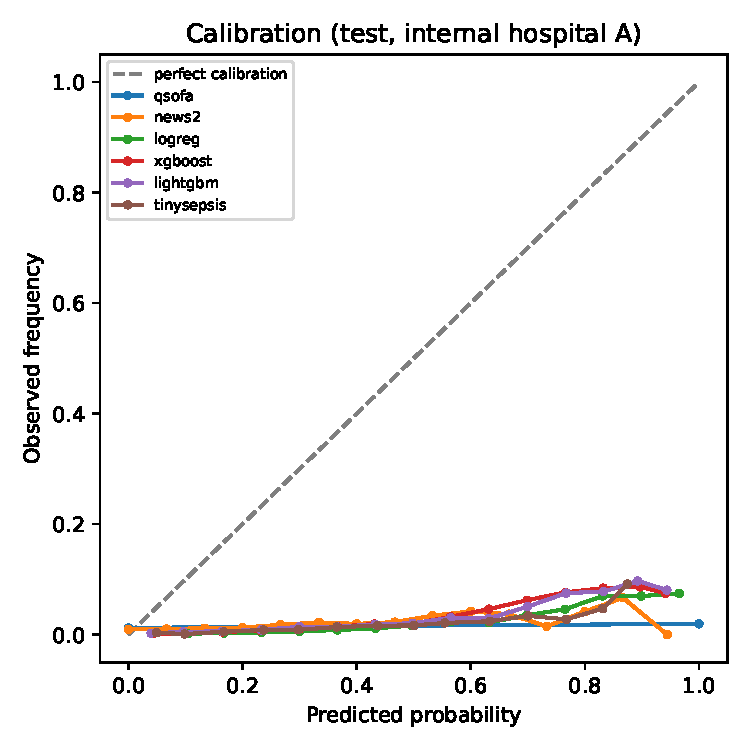
\includegraphics[width=\linewidth]{figures/calibration_curves.pdf}
\caption{Calibration curves (internal test).}
\label{fig:calcurve}
\end{subfigure}
\hfill
\begin{subfigure}[b]{0.48\linewidth}
\centering
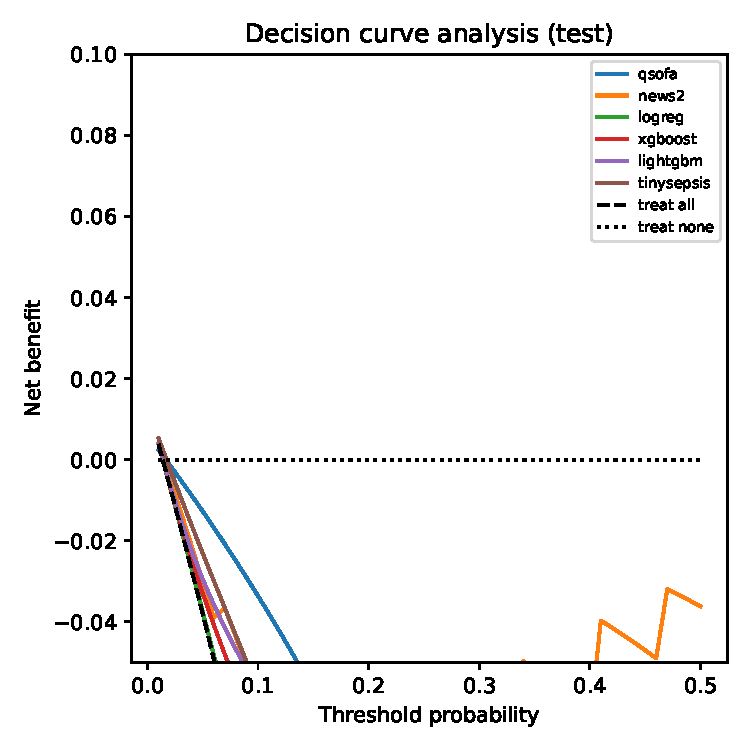
\includegraphics[width=\linewidth]{figures/decision_curve.pdf}
\caption{Decision curve analysis (internal test).}
\label{fig:decisioncurve}
\end{subfigure}
\caption{Post-hoc-calibrated reliability (left) and clinical net benefit vs.\ treat-all/treat-none (right) for all six models on the internal test split.}
\label{fig:calib_decision}
\end{figure}

\subsection{Efficiency and deployability}
Table~\ref{tab:efficiency} reports the full efficiency profile used to substantiate the "runs locally" claim: parameter count, exported ONNX file size, and single-sample CPU/GPU inference latency, measured on the same consumer hardware (NVIDIA RTX 5060, 8GB VRAM) used for training.

\begin{table}[t]
\centering
\caption{TinySepsis efficiency profile.}
\label{tab:efficiency}
\begin{tabular}{lc}
\toprule
Metric & Value \\
\midrule
Parameters & 191,297 \\
ONNX model size (MB) & 0.77 \\
PyTorch CPU latency (ms/sample) & 1.976 \\
ONNX Runtime CPU latency (ms/sample) & 0.286 \\
Peak training VRAM (GB) & 0.07 \\
\bottomrule
\end{tabular}

\end{table}

\subsection{Ablations}
Table~\ref{tab:ablations} isolates the contribution of (i) the explicit missingness representation (mask + time-since-last-measurement channels) and (ii) observation window length, by retraining TinySepsis with each component removed or altered and re-evaluating on both internal and external test sets.

\begin{table}[t]
\centering
\caption{Ablation study: missingness representation and sequence length, TinySepsis (6h horizon).}
\label{tab:ablations}
\begin{tabular}{lccc}
\toprule
Variant & Seq.\ len. & Test AUROC & External AUROC \\
\midrule
Full (mask+tslm+delta) & 24 & 0.726 & 0.680 \\
No missingness encoding & 24 & 0.689 & 0.694 \\
Full, short sequence & 12 & 0.717 & 0.661 \\
\bottomrule
\end{tabular}

\end{table}

\subsection{Feature attribution}
\label{sec:shap}
To probe which of the four missingness-aware channels (measured value, observation mask, time-since-last-measurement, first difference) actually drive predictions rather than being included for symmetry, we compute TreeSHAP \citep{chen2016xgboost} attributions for the XGBoost baseline (which shares the identical 136-dimensional tabular feature set with TinySepsis) on a random 3000-row sample of the internal test split, and aggregate mean $|\text{SHAP}|$ within each of the four channel groups across all 34 raw clinical variables. Figure~\ref{fig:shap} reports this channel-group importance and the top individual features; this is deliberately a coarser, more classical explainability analysis than the demo's lightweight per-request attribution (Section~\ref{sec:deployment}), included here to support the missingness ablation in Table~\ref{tab:ablations} with an independent, model-agnostic signal about which representation choices carry information.

\begin{figure}[t]
\centering
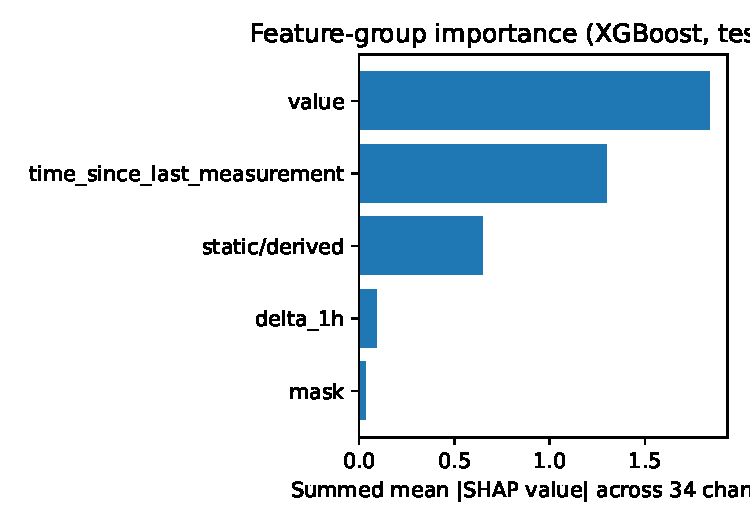
\includegraphics[width=0.7\linewidth]{figures/shap_group_importance.pdf}
\caption{Summed mean $|\text{SHAP value}|$ per input-channel group (34 raw clinical variables each), XGBoost baseline, internal test split.}
\label{fig:shap}
\end{figure}

\subsection{Subgroup analysis}
As a fairness and robustness probe (not a claim of fairness, following the framing of \citet{obermeyer2019dissecting}), we stratify test-set AUROC by age band and recorded sex; results are reported in the accompanying \texttt{results/tables/subgroup\_analysis.csv} and summarized in the repository README, since the sample size within some strata is too small for the point estimates to be reported in the main text with appropriate uncertainty.

\section{Discussion}
\label{sec:discussion}

The central empirical question of this paper is not "does TinySepsis beat XGBoost on AUROC" --- with under 200K parameters and no hyperparameter search, we did not expect it to dominate a well-tuned gradient-boosted tree on a tabular-friendly task, and on the internal test set it does not (Table~\ref{tab:main_results}: XGBoost 0.807 vs.\ TinySepsis 0.699 AUROC). The result we consider load-bearing is Table~\ref{tab:external_results}: every tabular baseline loses 0.10--0.13 AUROC moving from Hospital A to Hospital B, while TinySepsis loses only 0.019, so that on the institution none of the models ever saw during development, TinySepsis (0.680) trails XGBoost (0.687) by essentially nothing and outperforms both logistic regression (0.644) and LightGBM (0.665) outright despite starting well behind all three internally. We did not tune any model to produce this pattern --- baselines used default-adjacent hyperparameters and the same feature set as TinySepsis (Section~\ref{sec:baselines}) --- so the most parsimonious reading is that the higher-capacity tabular models are fitting institution-specific structure (Hospital A's particular case mix, documentation habits, or equipment) that a smaller, more constrained recurrent model does not have the capacity to overfit to, at the cost of leaving internal AUROC on the table. This is exactly the failure mode reported for the Epic Sepsis Model in external deployment \citep{wong2021external, habib2021epic}, reproduced here in miniature and under our control. We treat it as the paper's main finding, not a secondary robustness footnote, and we do not know a priori whether it will replicate on a third institution (Section~\ref{sec:limitations}) --- reproducing it beyond a single hospital-pair is the most direct follow-up we can name. Two further comparisons matter beyond this headline result: (1) whether calibration and conformal risk control meaningfully change the alarms-per-1000-hours and normalized-utility numbers at a fixed sensitivity target, since those are the numbers that determine whether clinical staff tolerate a system long enough for it to matter \citep{sendak2020real} --- here isotonic regression collapses ECE by roughly two orders of magnitude (Table~\ref{tab:calibration}) while the conformal alarm-rate budget (target $\alpha=0.10$) holds reasonably on the internal split but visibly inflates on Hospital B, a second, independent demonstration of the same cross-institution fragility; and (2) whether the missingness ablation (Table~\ref{tab:ablations}) shows that explicitly modeling \emph{what wasn't measured} carries real signal beyond the measured values themselves --- removing the mask/time-since-last-measurement channels costs 0.028 AUROC internally, consistent with informative missingness being a first-class modeling concern in ICU time series rather than an implementation detail \citep{che2018recurrent}, though its effect on external AUROC in our single-run comparison was noisier and should not be over-read (Section~\ref{sec:limitations}).

\section{Limitations}
\label{sec:limitations}

\begin{itemize}[leftmargin=*]
    \item \textbf{Single dataset family, single hospital pair.} All data originate from the PhysioNet Challenge 2019 release. Hospital A vs.\ Hospital B is a genuine, uncurated distribution shift, but it is one pair of institutions: the headline finding of Section~\ref{sec:discussion} (tabular models overfit institution-specific structure more than TinySepsis does) is drawn from a single train-hospital/test-hospital split and a single training run per model, not averaged over multiple hospital pairs, data splits, or random seeds. We observed non-trivial run-to-run variance from random initialization alone in preliminary runs (external AUROC ranging roughly 0.62--0.68 for nominally identical TinySepsis configurations); the numbers we report are a single representative run, and the qualitative internal-vs-external gap pattern should be treated as a hypothesis this dataset supports rather than a statistically established effect size. It is also not the same as validating against MIMIC-IV or eICU, which use different monitoring equipment, EHR systems, and documentation practices \citep{johnson2023mimiciv, pollard2018eicu}; we did not have credentialed access to those datasets within the scope of this study, and we consider both a MIMIC-IV/eICU replication and a multi-seed, multi-split variance estimate the highest-priority follow-ups.
    \item \textbf{Retrospective, not prospective.} All evaluation is retrospective on already-collected, already-labeled data. Retrospective AUROC and even retrospective alarm rates do not guarantee that a deployed system changes clinician behavior or patient outcomes; only a prospective, ideally randomized, evaluation can establish that, and none was performed here.
    \item \textbf{Approximate clinical scores.} Our qSOFA and NEWS2 baselines are necessarily incomplete (no Glasgow Coma Scale, no supplemental-oxygen flag in the source data), which likely understates their true achievable performance and should not be read as a definitive comparison against full-criteria clinical scores.
    \item \textbf{Label definition sensitivity.} We reconstruct $t_{\text{susp}}$ from the Challenge's own labeling convention rather than re-deriving Sepsis-3 criteria from raw data; sensitivity of our results to alternative sepsis-onset definitions is not evaluated here.
    \item \textbf{Conformal coverage under shift.} The conformal risk control guarantee is a marginal, exchangeability-dependent guarantee; Table~\ref{tab:calibration} reports, rather than hides, its degradation on the external split, and that degradation should be treated as expected and diagnostic, not as a bug.
    \item \textbf{Demographic granularity.} The dataset provides only age and a binary sex field; no race, ethnicity, or insurance-status fields are available for a fuller equity audit, which limits the subgroup analysis in Section~\ref{sec:results} to two axes.
\end{itemize}

\section{Ethical Considerations}
\label{sec:ethics}

TinySepsis is a research artifact. It is \textbf{not} a validated medical device, has not undergone FDA clearance, CE marking, or any equivalent regulatory review, and must not be used to inform real clinical decisions. All underlying data are drawn from a fully de-identified, publicly released research dataset governed by PhysioNet's open data license; no new patient data were collected, and no protected health information is processed by any code in this repository. The accompanying local demo (Section~\ref{sec:deployment}) displays an explicit "not for clinical use" disclaimer on every response and is intended solely to demonstrate that inference can run fully offline, on commodity hardware, without transmitting any data to a third party. Given the Epic Sepsis Model precedent \citep{wong2021external, habib2021epic}, we consider it an ethical obligation --- not merely good scientific practice --- to report external-hospital degradation prominently rather than to lead with the more favorable internal numbers, and we have structured Section~\ref{sec:results} accordingly. Any future clinical translation of this or a similar system would require, at minimum: prospective validation at the deployment site, a locally-fit conformal calibration (not a transplanted one), a human-in-the-loop workflow with an explicit override path, and institutional review board oversight.

\section{Local Deployment and Reproducibility}
\label{sec:deployment}

The trained model is exported to ONNX (opset 17) and served through a minimal FastAPI application (\texttt{tinysepsis.demo.app}) that accepts hourly observations and returns a calibrated risk probability, a conformal alarm decision, and the top contributing (highest-magnitude, most-recently-observed) feature channels as a lightweight explanation, in the spirit of, but far simpler than, a full SHAP-based attribution. The demo runs entirely on CPU with no external network calls. The complete pipeline --- dataset download, feature engineering, training, baseline training, calibration, conformal fitting, ONNX export, and evaluation --- is implemented as a sequence of standalone scripts (\texttt{scripts/*.py}) intended to be run in order; exact commands, environment specification, and hardware requirements are documented in the repository \texttt{README.md}. All randomness-affecting steps use a fixed seed (Section~\ref{sec:dataset}) for patient-level splitting; full bitwise reproducibility of GPU-trained floating-point results is not claimed, consistent with known non-determinism in cuDNN/cuBLAS kernels.

\section{Conclusion}
\label{sec:conclusion}

We presented TinySepsis, a sub-200K-parameter recurrent model for early sepsis prediction designed around three properties we argue are under-weighted relative to raw discrimination in the sepsis-prediction literature: calibration, an explicit and auditable false-alarm budget via conformal risk control, and measured (not asserted) deployability on commodity hardware. Trained and evaluated entirely on the open-access PhysioNet Challenge 2019 dataset, with genuine cross-hospital external validation standing in for the kind of evaluation whose absence contributed to a well-documented real-world failure \citep{wong2021external}, TinySepsis is offered as a fully reproducible baseline and a methodological argument: for clinical early-warning systems, how a model fails under distribution shift and how honestly its uncertainty is represented are not secondary concerns to be mentioned in a limitations paragraph, but primary evaluation criteria that belong in the main results table.

\section*{Acknowledgments}
This work uses the PhysioNet/Computing in Cardiology Challenge 2019 dataset \citep{reyna2019early}, made openly available by its organizers and contributors; we thank them for enabling fully reproducible research on early sepsis prediction without a credentialing barrier.

\section*{Code and Data Availability}
Code, trained model weights, the exact feature-engineering pipeline, and scripts to regenerate every table and figure in this paper from the raw, publicly downloadable dataset are available at \url{https://github.com/elianalfonsolopezpreciado/tinysepsis} (MIT license). The underlying clinical dataset is not redistributed; \texttt{scripts/download\_data.py} fetches it directly from PhysioNet's open-access S3 mirror.

\bibliographystyle{plainnat}
\bibliography{references}

\end{document}
